\documentclass[a4paper, 12pt]{scrartcl}
\usepackage{amsfonts}
\usepackage[a4paper]{geometry}
\usepackage{alltt}
\usepackage{lmodern}
\usepackage{amssymb}
\usepackage{mathtools}
\usepackage{amsmath}
\usepackage{enumerate}
\usepackage{float}
\usepackage{graphicx}
\usepackage{array}
\usepackage{listings}
\usepackage{fullpage}
\usepackage[parfill]{parskip}
\usepackage[utf8]{inputenc}
\usepackage[english]{babel}

\graphicspath{ {images/} }

\title{Space Rave Documentation}
\subtitle{Interactive Visual Computing WiSe 14/15}
\author{Arne Beer, MN 6489196\\
Rafael Epplee, MN 6269560\\
Sven-Hendrik Haase, MN 6341873}

\begin{document}
\maketitle \section{Introduction}

    For our IVC project ``Space Rave'', we set out to explore the emotional impact of a music video
    that is synchronized to the contemporary electronic dance music song ``Strobe'' by Deadmau5. We
    chose this song due to its regular profile and agreeable electronic character.  The video
    consists of three distinct scenes while the visuals are set to up to represent an abstract
    spacescape throughout the scenes. The visuals consist of procedurally generated stars which
    pulse rythmically and swiftly with every kick, a procedural, fluctuating background nebula and
    a tastefully hand-modelled spaceship.

    From a technical standpoint, we used POV-Ray to generated the images and Audacity to analyze
    the music to find beats and chords. The timings were particuarly hard to get right.

    It should be noted that while we do not own the rights to the song we used, we believe that we
    are using this song in good faith in our transformative work under Fair Use.

    \section{Extracting rythm information from the sound file}

    Since POV-Ray does come with any kind of Fourier transformation, we had to analyze the song by
    hand with Audacity. While this worked fairly well, we had to be very careful about the
    sub-second timings which are easy to offset by a few milliseconds which ruins the whole
    experience.

    \begin{figure}[H]
        \centering
        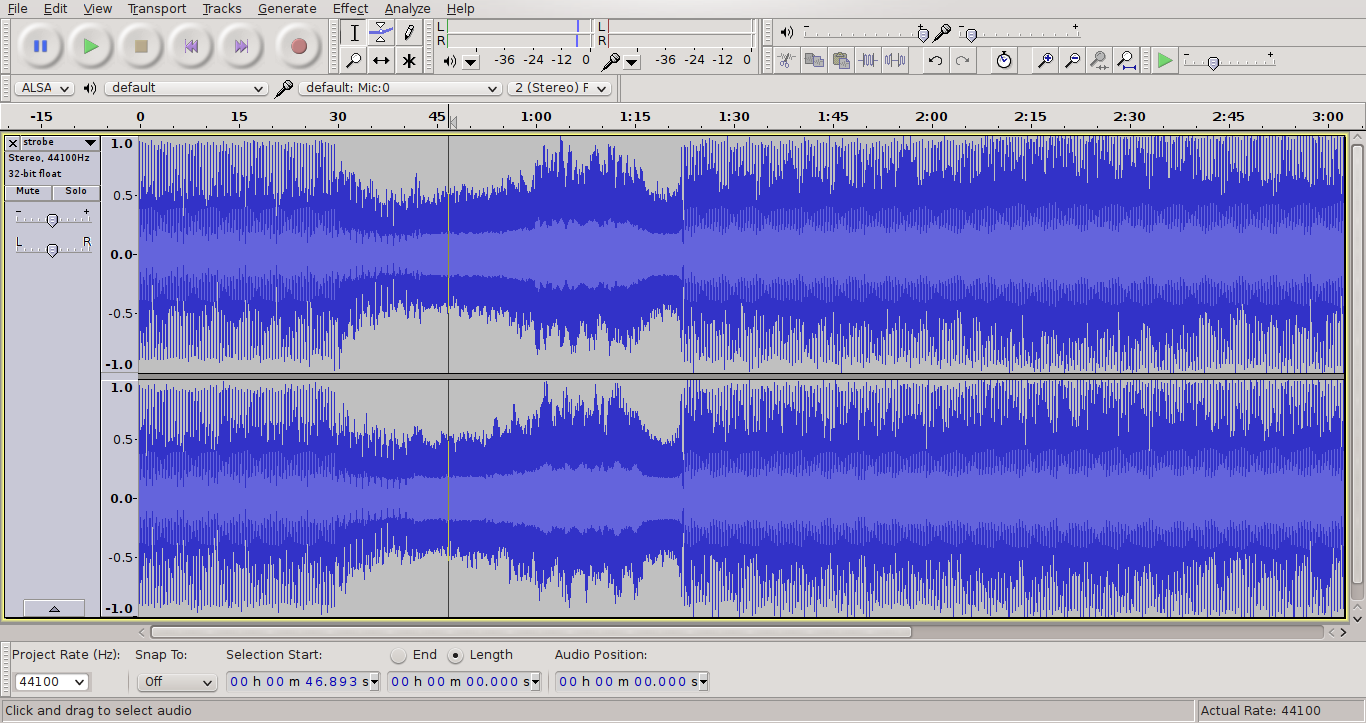
\includegraphics[scale=0.4]{audacity_main}
        \caption{Audacity main view of the track}
    \end{figure}

    \begin{figure}[H]
        \centering
        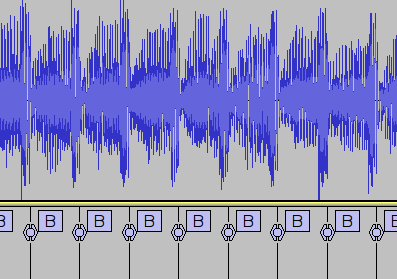
\includegraphics{audacity_beat}
        \caption{Beat analysis using Audacity's beat finder}
    \end{figure}

    \begin{figure}[H]
        \centering
        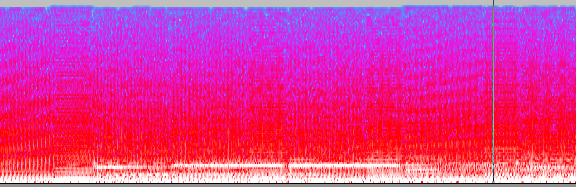
\includegraphics{audacity_spectrum}
        \caption{Spectrum view}
    \end{figure}

    \section{Spaceship Modeling}

    \section{Summary}

\end{document}
